\chapter{\IfLanguageName{dutch}{Stand van zaken}{State of the art}}%
\label{ch:stand-van-zaken}


% Tip: Begin elk hoofdstuk met een paragraaf inleiding die beschrijft hoe
% dit hoofdstuk past binnen het geheel van de bachelorproef. Geef in het
% bijzonder aan wat de link is met het vorige en volgende hoofdstuk.

% Pas na deze inleidende paragraaf komt de eerste sectiehoofding.

%Dit hoofdstuk bevat je literatuurstudie. De inhoud gaat verder op de inleiding, maar zal het onderwerp van de bachelorproef *diepgaand* uitspitten. De bedoeling is dat de lezer na lezing van dit hoofdstuk helemaal op de hoogte is van de huidige stand van zaken (state-of-the-art) in het onderzoeksdomein. Iemand die niet vertrouwd is met het onderwerp, weet nu voldoende om de rest van het verhaal te kunnen volgen, zonder dat die er nog andere informatie moet over opzoeken \autocite{Pollefliet2011}.

%Je verwijst bij elke bewering die je doet, vakterm die je introduceert, enz.\ naar je bronnen. In \LaTeX{} kan dat met het commando \texttt{$\backslash${textcite\{\}}} of \texttt{$\backslash${autocite\{\}}}. Als argument van het commando geef je de ``sleutel'' van een ``record'' in een bibliografische databank in het Bib\LaTeX{}-formaat (een tekstbestand). Als je expliciet naar de auteur verwijst in de zin (narratieve referentie), gebruik je \texttt{$\backslash${}textcite\{\}}. Soms is de auteursnaam niet expliciet een onderdeel van de zin, dan gebruik je \texttt{$\backslash${}autocite\{\}} (referentie tussen haakjes). Dit gebruik je bv.~bij een citaat, of om in het bijschrift van een overgenomen afbeelding, broncode, tabel, enz. te verwijzen naar de bron. In de volgende paragraaf een voorbeeld van elk.

%\textcite{Knuth1998} schreef een van de standaardwerken over sorteer- en zoekalgoritmen. Experten zijn het erover eens dat cloud computing een interessante opportuniteit vormen, zowel voor gebruikers als voor dienstverleners op vlak van informatietechnologie~\autocite{Creeger2009}.%


\section{Het belang van sales- en winstvoorspellingen}  

Een vraag die veel managers zich stellen, is waarom het zo belangrijk is om sales en winst te voorspellen. Zoals beschreven in Sales Forecasting Management van \textcite{JohnT.Mentzer2004}, is het antwoord simpel: elke keer dat er een plan wordt gemaakt, wordt er impliciet ook een voorspelling gemaakt. Dit geldt voor zowel individuen als organisaties en vormt de basis voor strategisch plannen. Wanneer een organisatie financiële plannen maakt op basis van verwachte verkoopcijfers, helpt een nauwkeurige voorspelling om deze doelen realistisch en haalbaar te maken. Slechte voorspellingen leiden dan ook tot slechte financiële plannen.


\section{Beperkingen van tijdsreeksen}  
Traditionele voorspellingsmethoden voor sales zijn vaak gebaseerd op tijdreeksen, dit betekent dat de vraag voor een product in het verleden kan gebruikt worden om de toekomstige vraag voor dit product te voorspellen. Deze methode werkt goed in markten waar de vraag stabiel blijft, maar kent beperkingen in meer dynamische markten. Het probleem is dat de vraag ook beïnvloed wordt door externe factoren zoals weersomstandigheden, economische ontwikkelingen, seizoensgebonden trends, consumentenvoorkeuren of zelfs veranderingen in het algemene sentiment. Tijdreeksen kunnen hier geen rekening mee houden, dit leidt tot minder nauwkeurige voorspellingen wanneer deze externe factoren groot zijn in belang. Een oplossing hiervoor zou een ander soort van voorspellingsmethoden zijn zoals causaal modelleren, met deze techniek kan je rekening houden met economische variabele, weersomstandigheden en marketingsstrategieën \autocite{UsugaCadavid2018}

\section{Vraag- en salesvoorspellingen}  
 

In de literatuur worden verschillende soorten voorspellingen onderscheiden volgens \textcite{UsugaCadavid2018}, zoals vraagvoorspellingen (demand forecasting) en sales voorspellingen (sales forecasting). In dit onderzoek wordt de focus gelegd op sales voorspellingen. Sales voorspelling is gebaseerd op gegevens die direct zijn verzameld uit verkooppunten, zoals winkeltransacties. Deze gegevens zijn gevoelig voor invloeden zoals promoties of voorraadtekorten, waardoor sales voorspellingen vaak de effectiviteit van promoties en de beschikbaarheid van producten weerspiegelen, in plaats van de werkelijke vraag. Aan de andere kant richt vraagvoorspelling zich op het identificeren van de werkelijke marktvraag, waarbij de effecten van promoties en voorraadtekorten zijn gecorrigeerd. Het doel is om een nauwkeuriger beeld te krijgen van de vraag, onafhankelijk van tijdelijke invloeden zoals marketingcampagnes of voorraadbeheer. Dit verschil, hoewel subtiel, heeft een grote invloed op de de manier waarop voorspellingen worden gemaakt en hoe bedrijven hun supply chain kunnen afstemmen op de werkelijke marktvraag in plaats van alleen verkoopaantallen .




\section{Strategische en praktische uitdagingen bij de integratie van Big Data}  
Big data biedt veel voordelen voor salesvoorspellingen, maar de integratie ervan is allesbehalve eenvoudig. \textcite{Boone2019} bespreken de strategische en praktische uitdagingen waarmee bedrijven worden geconfronteerd bij het incorporeren van big data in hun voorspellingsmodellen. Op strategisch niveau moet elk bedrijf beslissen of en hoeveel big data-technologieën ze willen integreren. Dit besluit hangt af van de potentiële voordelen van het gebruik van big data in vergelijking met de kosten van het verzamelen en analyseren van deze gegevens. 

\vspace{1 em}

Big data heeft het potentieel om productvoorspellingen te verbeteren en waardevolle inzichten te geven in klantgedrag. Echter, de praktische uitdaging van demand planners is de enorme hoeveelheid gegevens die verzameld wordt, zoals bijvoorbeeld de 2,5 petabytes aan data die Walmart elke uur verzamelt. De vraag die hierbij opkomt, is welke data bewaard moeten worden en hoe lang. 

\vspace{45 mm}

Een belangrijk obstakel bij het gebruik van big data voor vraagvoorspellingen is de invloed van menselijke beoordelingen. Veel bedrijven baseren hun voorspellingen op "gevoel" en passen statistische modellen aan op basis van factoren die vraagvoorspellers moeilijk kunnen meten zoals marketingactiviteiten of seizoenstrends. Hoewel menselijke beoordeling de voorspellingen kan verbeteren, introduceert het vaak vooroordelen die de nauwkeurigheid verminderen. Boone et al. suggereren dat big data mogelijk de negatieve effecten van deze "aanpassingen" kan verminderen, maar ze erkennen dat de praktische integratie van big data in ERP-systemen veel uitdagingen met zich meebrengt

\section{De evolutie van Big Data}  

Volgens \textcite{Lee2017} kan de evolutie van Big Data worden onderverdeeld in drie fasen. Hoewel het verzamelen en opslaan van gegevens al in de vroege jaren vijftig plaatsvond, met de introductie van de eerste commerciële mainframecomputers, heeft Big Data pas een exponentiële groei doorgemaakt sinds de uitvinding van het World Wide Web.


\subsection{Big Data 1.0: De opkomst van e-commerce}  

De eerste fase van Big Data, bekend als Big Data 1.0 (1994–2004) viel samen met de opkomst van e-commerce. In deze periode waren bedrijven de grootste aanbieders van webcontent, terwijl bijdragen van gebruikers slechts een kleine rol speelden vanwege de technische beperkingen van webapplicaties in die tijd. Om het online gedrag van gebruikers te analyseren, werden in deze fase web mining-technieken ontwikkeld, die onder te verdelen zijn in drie categorieën: web usage mining, web structure mining en web content mining.

\vspace{1 em}

Web usage mining richtte zich op het analyseren van hoe mensen websites gebruikten. Door gegevens over hun identiteit en surfgedrag, zoals muisklikken, zoekopdrachten en navigatiepatronen, te verzamelen, konden bedrijven hun diensten beter afstemmen op individuele gebruikers.

\vspace{1 em}

Web structure mining onderzocht de opbouw van websites door hyperlinks te analyseren, waardoor relaties tussen pagina’s zichtbaar werden en categorisering mogelijk werd. Een bekend voorbeeld hiervan was Google’s PageRank, dat deze links gebruikte om de relevantie en populariteit van pagina’s te bepalen.

\vspace{1 em}

Web content mining richtte zich op het verzamelen van informatie uit webpagina’s, zoals tekst, afbeeldingen, audio en video. Met technieken als tekstanalyse en natuurlijke taalverwerking (NLP) werden patronen herkend en pagina’s verdeeld, bijvoorbeeld om cyberterrorisme, e-mailfraude en spam te detecteren. Hoewel er destijds al methoden voor beeldverwerking bestonden, werden deze nog nauwelijks toegepast op web content mining.


\subsection{Big Data 2.0: De invloed van social media}  

De tweede fase van Big Data, bekend als Big Data 2.0 (2005–2014), werd aangedreven door de opkomst van social media. Gebruikers konden interacties hebben met de websites en met elkaar, en hun eigen content creëren en delen. Dit leidde tot een fundamentele verandering in de manier waarop bedrijven met klanten communiceren en samenwerken. Met social media analytics kunnen bedrijven inzicht krijgen in het gedrag van gebruikers op sociale mediaplatforms, zoals hun interesses, online activiteiten, vriendschappen, gevoelens en meningen. Deze inzichten stellen bedrijven in staat om effectievere marketingcampagnes te ontwikkelen.



\subsection{Big Data 3.0: De rol van IoT en streaming analytics}  

De laatste fase van Big Data volgens \textcite{Lee2017}, bekend als Big Data 3.0 (2015–heden), bouwt voort op de gegevens van Big Data 1.0 en Big Data 2.0. De kern van Big Data 3.0 wordt aangedreven door IoT-applicaties die data genereren in de vorm van video, audio en foto’s. Voor veel IoT-toepassingen wordt de analyse steeds vaker uitgevoerd door sensoren op de plaats waar de data wordt verzameld. Deze trend leidt tot een nieuw vakgebied, genaamd streaming analytics.



\section{Voorspellingsmodellen voor retaildata}  

In een onderzoek uitgevoerd door \textcite{Neba2024}  op een Walmart-dataset werd ontdekt dat traditionele lineaire modellen vaak niet in staat zijn om de complexe, niet-lineaire relaties binnen retaildata vast te leggen. Deze modellen konden de ingewikkelde interacties tussen verschillende variabelen niet effectief begrijpen. Aan de andere kant toonden geavanceerdere ensemble-methoden, zoals Random Forest en Gradient Boosting Machines (GBM), aanzienlijk betere voorspellende nauwkeurigheid door de uitkomsten van meerdere besluitbomen te combineren. Deze methoden wisten verborgen patronen te identificeren en de voorspellingsprecisie te verbeteren.

\vspace{1 em}

Van de geavanceerde modellen bleek XGBoost het beste te presteren, met de laagste Mean Absolute Error (MAE) en Root Mean Squared Error (RMSE). Dit onderstreepte de superieure capaciteiten van XGBoost voor het maken van nauwkeurige verkoopvoorspellingen. De verbeterde prestaties werden toegeschreven aan de efficiënte implementatie van gradient boosting, evenals aan technieken zoals regularisatie en het omgaan met ontbrekende waarden, waardoor XGBoost het model van keuze werd voor accurate verkoopvoorspellingen.

\vspace{10 mm}

\section{Klantsegmentatie}  

Volgens Pareto’s 80/20-regel is een klein percentage van de klanten vaak verantwoordelijk voor een groot deel van de omzet van een bedrijf. Hoewel dit principe in veel gevallen wordt waargenomen, is het belangrijk om op te merken dat dit niet altijd strikt van toepassing is. Dit betekent dat het behouden van deze klanten enorm belangrijk en soms zelf belangrijker als nieuwe klanten aantrekken. \textcite{Wu2011} benadrukken in hun onderzoek naar klantsegmentatie het belang van het begrijpen van klantgedrag. Ze stellen at bedrijven effectieve marketingstrategieën te ontwikkelen op basis van klantsegmenten, waarbij ze de koopgewoonten van klanten analyseren. 

\vspace{1 em}

Een natuurlijk gevolg van klantsegmentatie is dat je klanten beter kunt bedienen door prijzen of aanbiedingen aan te passen aan hun individuele behoeften. Deze aanpak maakt het mogelijk voor bedrijven om prijzen of aanbiedingen af te stemmen op de specifieke kenmerken en behoeften van individuele klanten, in plaats van gebruik te maken van algemene en uniforme strategieën.

\vspace{1 em}

Een van de grootste voordelen van een gepersonaliseerde benadering is de positieve invloed op klantbehoud. Klanten die het gevoel hebben dat producten of diensten eerlijk en relevant zijn voor hun situatie, blijven loyaal aan het bedrijf. Daarnaast versterkt personalisatie het vertrouwen van klanten, doordat zij het gevoel krijgen als individu te worden behandeld in plaats van slechts een nummer in een database te zijn. Zo kunnen bijvoorbeeld trouwe klanten beloond worden met speciale aanbiedingen of kortingen, wat hun loyaliteit versterkt. Daarentegen kan een niet-gepersonaliseerde aanpak ervoor zorgen dat klanten zich niet gewaardeerd voelen of het idee krijgen dat ze te veel betalen. Dit vergroot de kans dat ze overstappen naar een concurrent, wat uiteindelijk kan resulteren in een hoger klantverloop.\autocite{Adeniran2024}


\section{Voorspellingen met Articiele intelligentie}  

Binnen de term van AI hebben we verschillende subcategorieën die gebruikt worden om voorspellingen te maken op basis van data. Twee van de belangrijkste hiervan zijn machine learning (ML) en deep learning (DL). ML maakt gebruik van algoritmes die patronen herkennen in data en deze toepassen voor voorspellingen, met technieken zoals supervised learning, unsupervised learning en reinforcement learning. Deep learning, een meer geavanceerde vorm van ML, gebruikt complexe neurale netwerken met meerdere lagen om nog diepere patronen te ontdekken, vooral bij ongestructureerde data zoals afbeeldingen of teksten. Beide technieken zijn essentieel voor het doen van nauwkeurige voorspellingen.

\begin{figure}[H]
    \centering
    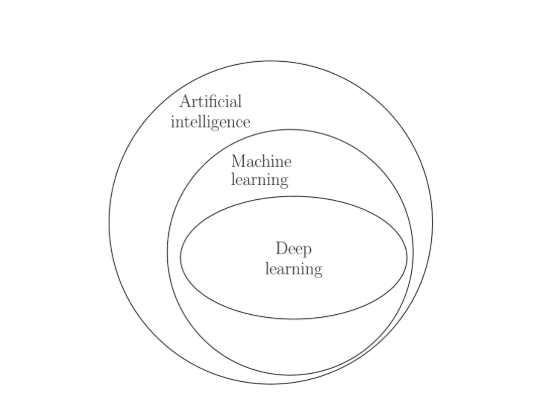
\includegraphics[width=0.7\linewidth]{images/RelatieAI_ML_DL}
    \caption{Relatie tussen AI, ML, en DL  (\cite{Kelleher2019})}
    \label{fig:relatieaimldl}
\end{figure}

\subsection{Machine learning}

Machine learning kan verder onderverdeeld worden in verschillende categorieën, zoals supervised learning, unsupervised learning en reinforcement learning.

\subsection*{Unsupervised learning}

Bij unsupervised learning krijgt het systeem alleen ongelabelde data. Het doel zoals vernoemd werd in \textcite{Naeem2023} is dat het systeem zelf patronen, structuren of groepen in de data ontdekt zonder dat er vooraf een specifieke taak of label is gedefinieerd. Een voorbeeld hiervan is het automatisch groeperen van foto’s van katten zonder dat de foto’s als zodanig zijn gemarkeerd.

\subsection*{Reinforcement learning}

In reinforcement learning leert een systeem door interacties met zijn omgeving, waarbij het probeert acties te ondernemen die de hoogste beloning oplevert. Dit proces wordt gestuurd door de "reward function", die bepaalt wat als goed of slecht wordt beschouwd voor het systeem. De reward function is vast en kan niet worden aangepast door het systeem zelf. Zoals in \textcite{Gallistel1999} vernoemd werd, helpt deze functie het systeem te sturen in het vinden van de beste strategie om zijn prestaties te verbeteren.


\vspace{20 mm}

\subsection*{Supervised learning}

Supervised Learning is een techniek binnen machine learning waarbij een model wordt getraind met gelabelde data. Het leert patronen te herkennen in de gegevens om vervolgens voorspellingen te doen voor nieuwe, onbekende data. Volgens \textcite{Fabris2017} maakt supervised machine learning gebruik van de kenmerken en annotaties in de trainingsset om een model te ontwikkelen dat de annotaties van de testset kan voorspellen. Deze methode is niet alleen nuttig voor voorspellingen, maar kan ook helpen bij het ontdekken van interpreteerbare kennis. Een voorbeeld hiervan is het classificeren van eiwitten als verouderingsgerelateerd (bron).

\subsection{Regressie modellen}

Regressiemodellen worden gebruikt om de relatie tussen een afhankelijke variabele en één of meer onafhankelijke variabelen te begrijpen. Het doel is om een voorspelling te doen over de afhankelijke variabele op basis van de waarden van de andere variabelen. Regressie wordt vaak gebruikt om trends te analyseren en toekomstige uitkomsten te voorspellen.

\subsection*{Random Forest}
Het Random Forest-model is een krachtig en populair machine learning-model dat wordt gebruikt voor zowel classificatie als regressie. Het algoritme maakt gebruik van een verzameling besluitbomen (decision trees) die willekeurig worden gegenereerd — vandaar de naam Random Forest. Elke boom in het model wordt opgebouwd op basis van een willekeurige selectie van features bij elk knooppunt. Deze willekeurigheid zorgt voor variatie tussen de bomen, waardoor het risico op overfitting afneemt en de nauwkeurigheid van het model toeneemt. Volgens \textcite{Sekhar2016} kan je het random forrest proces in de volgende stappen opsplitsen:



\subsection*{Support Vector Machine}

Volgens \textcite{RodriguezPerez2022} zijn Support Vector Machine (SVM) is een krachtig machine learning algoritme dat oorspronkelijk werd ontwikkeld door Vapnik in 1979. Het algoritme werd eerst ontworpen voor binaire classificatieproblemen, waarbij het doel is om objecten in twee categorieën te verdelen. Later werd het uitgebreid naar regressieproblemen, wat bekend staat als Support Vector Regression (SVR).

\vspace{1em}

Wat SVM onderscheidt van andere algoritmes is de manier waarop het werkt met data. Het algoritme projecteert de trainingsdata in een vooraf gedefinieerde feature space, waarin het op zoek gaat naar een hypervlak dat de verschillende klassen optimaal van elkaar scheidt. Als zo’n scheiding in de oorspronkelijke ruimte niet mogelijk is, dan wordt de data getransformeerd naar een ruimte met hogere dimensies waar een lineaire scheiding wél haalbaar kan zijn.

\vspace{1em}

Een belangrijk aspect van SVM is het gebruik van de zogenaamde soft margin variant. Deze laat toe dat sommige punten aan de verkeerde kant van het hypervlak liggen om zo een beter generaliserend model te bekomen. Dit maakt SVM robuuster voor data die niet perfect lineair scheidbaar zijn.

\subsection*{Lineaire regressie}

Lineaire regressie is een veelgebruikte en eenvoudige methode om verbanden tussen meerdere variabelen te analyseren en voorspellingen te doen. Het model wordt vaak toegepast vanwege de duidelijkheid en controle die het biedt in vergelijking met complexere machine learning-modellen.\autocite{Etemadi2021}
\vspace{1em}

Lineaire regressie onderzoekt hoe veranderingen in een afhankelijke variabele verklaard kunnen worden door meerdere onafhankelijke variabelen. Dit kan voor twee doelen worden ingezet:


Deze methode wordt breed toegepast in domeinen zoals geneeskunde, techniek, energie, financiën en milieuwetenschappen. Zo werd lineaire regressie bijvoorbeeld gebruikt om COVID-19 trends te voorspellen, luchtvervuiling te koppelen aan ziekenhuisopnames, en energieverbruik in gebouwen te schatten.

\vspace{1em}

Dankzij zijn eenvoud en flexibiliteit blijft lineaire regressie een krachtig hulpmiddel voor zowel verklarende als voorspellende analyses.


\subsection*{XGBoost}

XGBoost is een krachtig en efficiënt algoritme voor machine learning dat gebaseerd is op het principe van gradient boosting. Het is ontworpen om snel en schaalbaar te zijn, waardoor het goed presteert op grote en complexe datasets. Het model werkt door meerdere eenvoudige beslissingsbomen te combineren. Elke nieuwe boom probeert de fouten van de vorige te verbeteren, waardoor het model stapsgewijs steeds nauwkeuriger wordt. Dankzij optimalisaties zoals parallelle verwerking en slimme technieken om het leerproces te versnellen, is XGBoost een populaire keuze.\autocite{Hakkal2024}

\subsection{Forecast modellen}

Forecast modellen zijn technieken die worden gebruikt om toekomstige waarden te voorspellen op basis van historische gegevens. Ze houden rekening met patronen zoals trends en seizoensgebonden fluctuaties voor nauwkeurige voorspellingen te doen.

\subsection*{SARIMA}

SARIMA is een voorspellingsmodel dat wordt gebruikt om tijdsreeksen te analyseren en toekomstige waarden te schatten. Het is een uitbreiding van het ARIMA-model, dat kijkt naar patronen in de vroegere waarden van een reeks. ARIMA werkt goed voor data zonder duidelijke seizoensinvloeden, maar wanneer er wél sprake is van terugkerende patronen, zoals elke maand of elk kwartaal, is SARIMA beter geschikt \autocite{KumarDubey2021}.

\vspace{1em}

SARIMA bestaat uit twee delen: een niet-seizoensgebonden deel (ARIMA) en een seizoensgebonden uitbreiding. Het model gebruikt verschillende parameters om de juiste voorspelling te maken. Zo geeft het aan hoeveel eerdere waarden (lags) gebruikt worden, hoeveel keer het verschil moet worden genomen om de data stabiel te maken, en hoeveel fouten uit het verleden worden meegenomen.

\vspace{1em}

Het maken van een SARIMA-model gebeurt in een aantal stappen. Eerst wordt gecontroleerd of de data stabiel is (stationair), wat betekent dat het gemiddelde en de spreiding niet veranderen over tijd. Als dat niet zo is, wordt de reeks aangepast door er verschillen van te nemen, net zo lang tot deze stabiel is. Daarna worden er modellen opgebouwd met behulp van patronen in de data. Pas als dat klaar is, kan de voorspelling gemaakt worden. Tot slot wordt gecontroleerd of de voorspelling klopt door de uitkomsten te vergelijken met echte waarden.

\vspace{1em}

SARIMA is handig voor situaties waarin je wilt voorspellen op basis van herhalende patronen in de tijd, zoals verkoop per maand of temperatuur per seizoen \autocite{KumarDubey2021}.

\subsection{Segmentatie modellen}

Segmentatiemodellen worden gebruikt om een groep op te delen in kleinere, vergelijkbare groepen. Dit helpt om patronen te vinden en gerichte acties te ondernemen voor verschillende groepen.

\subsection*{K-means}

Volgens \textcite{Hu2023} is K-means een populaire techniek voor het clusteren van gegevens, waarbij een verzameling van n observaties wordt verdeeld in k groepen. Elk gegevenspunt wordt toegewezen aan de groep waarvan het centrum het dichtstbij ligt. Dit proces gaat door totdat de posities van de centroïden stabiel blijven en de variatie binnen de clusters geminimaliseerd is. Het algoritme werkt iteratief: in de eerste stap worden de punten aan een willekeurig gekozen centrum toegewezen. Vervolgens worden de centra aangepast op basis van de nieuwe groepering, en dit proces wordt herhaald totdat de indeling niet meer verandert.

\subsection*{K-modes}

Het K-modes algoritme volgens \textcite{Kuo2021} is een clustering-algoritme dat specifiek is ontwikkeld voor categorische data. Het is een aanpassing van het K-means algoritme. De belangrijkste verschillen tussen K-means en K-modes zijn:



K-modes is ideaal voor datasets met alleen categorische gegevens, omdat het beter past bij de eigenschappen van deze variabelen en helpt bij het ontdekken van patronen die moeilijk te clusteren zouden zijn met traditionele methoden.

\subsection*{DBScan}

DBSCAN is volgens \textcite{Hanafi2022} een bekend en veelgebruikt algoritme dat groepen maakt op basis van hoe dicht punten bij elkaar liggen. In vergelijking met andere methodes om data te groeperen, heeft DBSCAN enkele sterke punten. Zo kan het groepen herkennen die niet netjes rond of vierkant zijn, het kan losse of afwijkende punten makkelijk opsporen, en het bepaalt automatisch hoeveel groepen er zijn zonder dat je dat vooraf hoeft aan te geven.

\vspace{1em}

Toch heeft DBSCAN ook nadelen. Een belangrijk probleem is dat het traag werkt bij grote hoeveelheden data. Hoe meer gegevens er zijn, hoe langer het duurt om voor elk punt te bepalen welke andere punten in de buurt liggen en hoe dicht die bij elkaar zitten. Hierdoor is het belangrijk om manieren te zoeken om DBSCAN sneller te laten werken, zodat het ook geschikt blijft voor grote datasets.

\vspace{1em}

Het algoritme werkt als volgt: DBSCAN begint met een willekeurig punt uit de dataset dat nog niet eerder is bekeken. Daarna wordt gekeken hoeveel andere punten er binnen een bepaalde afstand (ε) van dit punt liggen. Als er te weinig punten dichtbij liggen (minder dan een minimum aantal, MinPts), wordt het punt gezien als ruis. Ligt het aantal wel boven die grens, dan wordt het punt een kernpunt en begint het algoritme een nieuwe cluster.

Alle punten die in de buurt liggen van dit kernpunt worden verzameld in een lijst. Voor elk van deze punten wordt opnieuw gekeken of het ook een kernpunt is. Als dat zo is, worden zijn buren ook toegevoegd aan de lijst, zodat de cluster zich verder uitbreidt. Als een punt geen kernpunt is, krijgt het alleen het label van de cluster maar wordt er niet verder gezocht vanuit dat punt. Dit proces gaat door tot de lijst leeg is. Daarna kiest het algoritme opnieuw een willekeurig punt dat nog niet is bekeken en herhaalt het proces, tot alle punten in de dataset zijn behandeld.\autocite{Hanafi2022}

\subsection{Deep learning}

Deep learning is een subcategorie binnen Artificial Intelligence die zich richt op het ontwikkelen van grote neurale netwerken die in staat zijn om nauwkeurige beslissingen te nemen. Deep learning is best geschikt voor situaties waar de data complex is en grote datasets beschikbaar zijn. Vandaag de dag maken de meeste online bedrijven gebruik van deep learning. Voorbeelden hiervan zijn Facebook, dat deep learning gebruikt om tekst in online gesprekken te analyseren, en Google, dat deep learning inzet voor afbeeldingszoekopdrachten. Moderne smartphones bevatten deep learning-systemen voor toepassingen zoals gezichtsherkenning en spraakherkenning. \autocite{Kelleher2019}

%\begin{figure}
%  \centering
%  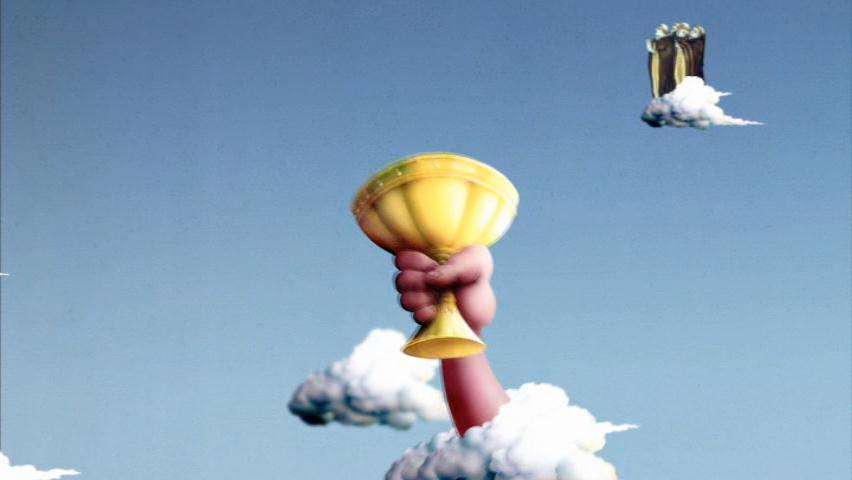
\includegraphics[width=0.8\textwidth]{grail.jpg}
%  \caption[Voorbeeld figuur.]{\label{fig:grail}Voorbeeld van invoegen van een figuur. Zorg altijd voor een uitgebreid bijschrift dat de figuur volledig beschrijft zonder in de tekst te moeten gaan zoeken. Vergeet ook je bronvermelding niet!}
%\end{figure}



%\begin{listing}
%%  \begin{minted}{python}
%%    import pandas as pd
%%    import seaborn as sns
%
%   % penguins = sns.load_dataset('penguins')
% %   sns.relplot(data=penguins, x="flipper_length_mm", y="bill_length_mm", hue="species")
%  %\end{minted}
%  \caption[Voorbeeld codefragment]{Voorbeeld van het invoegen van een codefragment.}
%\end{listing}






%\begin{table}
%  \centering
%  \begin{tabular}{lcr}
%    \toprule
%    \textbf{Kolom 1} & \textbf{Kolom 2} & \textbf{Kolom 3} \\
%    $\alpha$         & $\beta$          & $\gamma$         \\
%    \midrule
%    A                & 10.230           & a                \\
%    B                & 45.678           & b                \\
%    C                & 99.987           & c                \\
%    \bottomrule
%  \end{tabular}
%  \caption[Voorbeeld tabel]{\label{tab:example}Voorbeeld van een tabel.}
%\end{table}

